%%%%%%%% ICML 2022 EXAMPLE LATEX SUBMISSION FILE %%%%%%%%%%%%%%%%%

\documentclass[nohyperref]{article}

% Recommended, but optional, packages for figures and better typesetting:
\usepackage{microtype}
\usepackage{graphicx}
\usepackage{subcaption}
\usepackage{booktabs} % for professional tables

% hyperref makes hyperlinks in the resulting PDF.
% If your build breaks (sometimes temporarily if a hyperlink spans a page)
% please comment out the following usepackage line and replace
% \usepackage{icml2022} with \usepackage[nohyperref]{icml2022} above.
\usepackage{hyperref}


% Attempt to make hyperref and algorithmic work together better:
\newcommand{\theHalgorithm}{\arabic{algorithm}}

% Use the following line for the initial blind version submitted for review:
\usepackage{icml2022}

% If accepted, instead use the following line for the camera-ready submission:
% \usepackage[accepted]{icml2022}

% For theorems and such
\usepackage{amsmath}
\usepackage{amssymb}
\usepackage{mathtools}
\usepackage{amsthm}

% if you use cleveref..
\usepackage[capitalize,noabbrev]{cleveref}

%%%%%%%%%%%%%%%%%%%%%%%%%%%%%%%%
% THEOREMS
%%%%%%%%%%%%%%%%%%%%%%%%%%%%%%%%
\theoremstyle{plain}
\newtheorem{theorem}{Theorem}[section]
\newtheorem{proposition}[theorem]{Proposition}
\newtheorem{lemma}[theorem]{Lemma}
\newtheorem{corollary}[theorem]{Corollary}
\theoremstyle{definition}
\newtheorem{definition}[theorem]{Definition}
\newtheorem{assumption}[theorem]{Assumption}
\theoremstyle{remark}
\newtheorem{remark}[theorem]{Remark}

% Todonotes is useful during development; simply uncomment the next line
%    and comment out the line below the next line to turn off comments
%\usepackage[disable,textsize=tiny]{todonotes}
\usepackage[textsize=tiny]{todonotes}


% The \icmltitle you define below is probably too long as a header.
% Therefore, a short form for the running title is supplied here:
\icmltitlerunning{One Datapoint is Not Enough: Disentangling Grouped Data with Confounding}

\begin{document}

\twocolumn[
\icmltitle{One Datapoint is Not Enough: Disentangling Grouped Data with Confounding}

% It is OKAY to include author information, even for blind
% submissions: the style file will automatically remove it for you
% unless you've provided the [accepted] option to the icml2022
% package.

% List of affiliations: The first argument should be a (short)
% identifier you will use later to specify author affiliations
% Academic affiliations should list Department, University, City, Region, Country
% Industry affiliations should list Company, City, Region, Country

% You can specify symbols, otherwise they are numbered in order.
% Ideally, you should not use this facility. Affiliations will be numbered
% in order of appearance and this is the preferred way.
% \icmlsetsymbol{equal}{*}

\begin{icmlauthorlist}
\icmlauthor{Dan Andrei Iliescu}{cam}
\icmlauthor{Damon J Wischik}{cam}
\end{icmlauthorlist}

\icmlaffiliation{cam}{Department of Computer Science, University of Cambridge, UK}

\icmlcorrespondingauthor{Dan Andrei Iliescu}{dai24@cam.ac.uk}

% You may provide any keywords that you
% find helpful for describing your paper; these are used to populate
% the "keywords" metadata in the PDF but will not be shown in the document
\icmlkeywords{Machine Learning, ICML}

\vskip 0.3in
]

% this must go after the closing bracket ] following \twocolumn[ ...

% This command actually creates the footnote in the first column
% listing the affiliations and the copyright notice.
% The command takes one argument, which is text to display at the start of the footnote.
% The \icmlEqualContribution command is standard text for equal contribution.
% Remove it (just {}) if you do not need this facility.

%\printAffiliationsAndNotice{}  % leave blank if no need to mention equal contribution
\printAffiliationsAndNotice{\icmlEqualContribution} % otherwise use the standard text.

\begin{abstract}
Group-instance disentanglement is the problem of learning separate representations for within-group and across-group variation. We introduce the Context-Aware Variational Autoencoder (CxVAE), a method which can perform group-instance disentanglement on datasets with confounding (i.e. where a single observation is not sufficient to accurately infer the group and instance variables). First, we generate a dataset with confounding that cannot be disentangled by the current state-of-the-art methods. Next, we improve upon these methods by proposing 3 modifications: 1) conditioning the instance variable on the group variable, 2) a more expressive group encoder, 3) a regularization objective that encourages independence between the instance variable and the grouping. Our method shows considerable gains in performance measured by several disentanglement metrics: holdout reconstruction error, unsupervised translation error, and latent code probing. Finally, we explore how adjusting the parameters of the data-generating process affects the performance gap between CxVAE and the state-of-the-art.
\end{abstract}

\section{Introduction}
\label{intro}

\begin{figure}[t]
    \vskip 0.2in
    \begin{center}
    \centerline{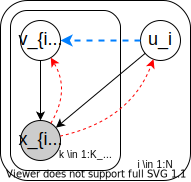
\includegraphics[width=0.7\columnwidth]{files/bayes_net_one.pdf}}
    \caption{\textbf{Group-Instance Generative Model.} For each group $i$, a group variable$u_i$ and a set of instance variables $\mathbf{v}$ generates the set of observations $\mathbf{x}$. The conditional $q(v_{ik} | u_i)$ (\textbf{blue arrow}) is absent from the existing literature but present in our proposed variational model. This enables our model to accurately infer the instance variable even when the groups are confounded. }
    \label{fig:pgm}
    \end{center}
    \vskip -0.2in
\end{figure}

Group-instance disentanglement is the task of learning a representation network $r(\mathbf{x})$ which transforms a group of observations $\mathbf{x} = \{x_1, ..., x_K\}$ (e.g. images grouped by author,  temperature readings grouped by weather station,  etc) into a \textit{group} code $u$ and a set of \textit{instance} codes $\mathbf{v} = \{v_1, ..., v_K\}$. The goal is that the group code should capture all the information that distinguishes one group from another,  while the instance code should capture all the information that distinguishes the observations within a group, but none of the group information.

The standard model for this task is the \textit{Group-Instance Generative Model} (GIGM) \citep{Bouchacourt2018MultiLevelVA, Hosoya2019GroupbasedLO}, depicted in \cref{fig:pgm}. The model treats group and instance as independent latent variables involved in the generation of the data.  We, in common with existing methods, train this model following the Variational Auteoncoder paradigm \citep{Kingma2014AutoEncodingVB,JimenezRezende2014StochasticBA}. In this framework, disentanglement is a property of the variational latent posterior $q(u, \mathbf{v} | \mathbf{x})$ which is implemented as a representation network.

Implementing the variational latent posterior so that it learns disentangled representations is not trivial and there exist several approaches. Challenges include how to accumulate evidence from multiple observations in order to infer the group variable \citep{Bouchacourt2018MultiLevelVA, Hosoya2019GroupbasedLO} and how to design a regularization objective that encourages disentanglement in practice \citep{Nmeth2020AdversarialDW}. 

Many datasets require that the inference model be able to capture the joint distribution between the group and instance variables conditioned on the observations. These are datasets where two identical observations could have come from different groups, and thus have different instance factors. We call these datasets \textit{with confounding} because in the data-generating process $u$ is a confounding variable when estimating $v$ from $x$. 

Such datasets are very common. For example, the problem of soybean plant growth \citep{Davidian1995NonlinearMF} has a dataset with confounding. It is impossible to deduce the age (instance) of a plant based solely on its leaf weight (observation) without also knowing its genotype (group). 

We show empirically that the state-of-the-art methods fail to learn disentangled representations on datasets with confounding.We generate a simple dataset of student exam scores grouped by school.  The instance variable captures the score of a student in relation to the distribution of scores at their school. Instead of disentangling, the existing methods split the representation of the group factor across both group and instance variables. 

In order to tackle this challenge, we propose the Context-Aware Variational Autoencoder (CxVAE), another approach to the GIGM model with several novel modifications. The main novelty is an instance encoder conditioned on the inferred group variable, which enables the variational latent posterior to match the full generative latent posterior.  Additionally, we use an expressive Deep Set network \citep{Zaheer2017DeepS} to infer the group variable more accurately, and also design a novel regularization objective that encourages independence between the inferred instance variable and the ground-truth group factor. 

We present the following contributions:
\begin{enumerate}
    \item We formalize the notion of datasets with confounding and generate a simple dataset on which the current group-instance methods fail to learn disentangled representations.
    \item We propose a new model, called the Context-Aware Variational Autoencoder (CxVAE) which can learn disentangled representations on emergent groups.
    \item We perform extensive evaluation showing that our model outperforms the existing methods in holdout-data log-likelihood, unsupervised translation, and ground-truth factor prediction.
    \item We complete an ablation study showing the relative performance gain brought by each modification of our model.
    \item By varying the amount of confounding in the data-generating process, we show that confounding explains the performance gain of the CxVAE over existing methods. We also show how different magnitude ratios between the group and instance factors affect disentanglement.
\end{enumerate}

\section{Generative Group-Instance}

The Group Variational Autoencoder \citep{Bouchacourt2018MultiLevelVA,Hosoya2019GroupbasedLO} is a family of models that use two latent variables to represent grouped data: one that captures the variation within groups, and one for the variation across groups.

Assume a dataset of the form $\{x_{ik}\}_{i \in 1:N, ~k \in 1:K_i}$ where $N$ is the number of groups and $K_i$ is the number of observations in group $i$. GVAE defines a generative model that maps a $\mathcal{N} (0,1)$ group latent variable $u_i$ and a $\mathcal{N} (0,1)$ instance latent variable $v_{ik}$ to a given data observation $x_{ik}$. In other words, the likelihood of a group is:

$$p(\mathbf{x}) = \mathbb{E}_{p(u)}  \prod_{k=1}^{K} \mathbb{E}_{p(v_{k})} ~ [p(x_{k} | u, v_{k})]$$

We omit the index of the group $i$ for notational simplicity, since the groups are independent and identically distributed.

\subsection{Variational Inference}

Because the exact likelihood is intractable, the Variational Autodencoder \citep{Kingma2014AutoEncodingVB,JimenezRezende2014StochasticBA} performs optimization by introducting a variational latent posterior $q(u, \mathbf{v} | \mathbf{x})$ and maximizing the Evidence Lower Bound \citep{Jordan2004AnIT}:

$$\log p(\mathbf{x}) \geq \mathbb{E}_{q(u, \mathbf{v} | \mathbf{x})} [\log p(\mathbf{x} | u, \mathbf{v})] - \mathrm{KL} [q(u, \mathbf{v} | \mathbf{x}) || p(u, \mathbf{v})]$$

\textit{Existing methods use a class of variational distributions that assume independence between the latent variables in a group when conditioned on the data.}

$$q(u, \mathbf{v} | \mathbf{x}) = q(u | \mathbf{x}) \prod_{k=1}^K q(v_k | x_k)$$

In our work, we show that this assumption hinders disentanglement when the generative model is entangled.

\subsection{Group Encoder}

We, in common with existing methods, implement the variational group posterior with normal density with $(\mu, \Sigma)$ computed with an encoder network. The way to implement the encoder network is not obvious, since the number of inputs $K$ varies across groups. \citet{Hosoya2019GroupbasedLO} encode separately each observation in the group using the same encoder $E_u$ to produce $\mu_k, \Sigma_k$ and then averages the outputs.

$$\mu = \frac{1}{N} \sum_{k=1}^K \mu_k, ~ \Sigma = \frac{1}{N} \sum_{k=1}^K \Sigma_k$$

\citet{Bouchacourt2018MultiLevelVA} also encode each observation individually and then accumulate the evidence through a product of normal densities, computed using the following equations:

$$\Sigma^{-1} = \sum_{k=1}^K \Sigma_k^{-1}, ~ \mu^T \Sigma^{-1} = \sum_{k=1}^K \mu_k^T \Sigma_k^{-1}$$

They justify that such a product of normals produces a valid evidence accumulation using the following result:

$$q(u | \mathbf{x}) \propto \prod_{k=1}^K q(u | x_k)$$

However, the above is not a universal property, since

\begin{align}
    \begin{split}
        q(u | \mathbf{x}) = &\frac{\prod_{k=1}^K q(x_k)}{q(\mathbf{x})} \frac{1}{q(u)^{K-1}} \prod_{k=1}^K q(u | x_k) \\ &\propto \frac{1}{q(u)^{K-1}} \prod_{k=1}^K q(u | x_k)
    \end{split}
\end{align}

In fact, by using a product of normals to accumulate evidence, the authors implicitly assume that the marginal distribution of the inferred group variable is a uniform. This has the effect of sampling $u$ values which are less representative of the current group and more skewed towards the marginal distribution of $u$.

In our work, we propose a more general approach to encoding $u$ by using a Deep Sets  network \citep{Zaheer2017DeepS} to encode the whole set of observations instead of encoding each observation separately.

\subsection{Regularization}

In certain cases, the model might learn to encode both kinds of variation (within- and across-group) in the instance variable, effectively turning the model into a standard VAE. In this eventuality, the group variable becomes irrelevant and disentanglement is not achieved.

Such behaviour has been identified by \citet{Hosoya2019GroupbasedLO} and \citet{Nmeth2020AdversarialDW} to occur when the instance code too high-dimensional, the instance encoder too expressive, or group sizes too small. One solution is to limit the dimensionality of the instance code \citep{Hosoya2019GroupbasedLO}, with the downside of hindering the overall model performance. 

As a more targeted solution, \citet{Hosoya2019GroupbasedLO} propose an adversarial loss minimizing the mutual information between an observation and the instance variable inferred from the other observations in the group:

$$I_{r} (x, v) = \mathrm{KL} [r(x, v) || r(x) r(v)]$$

where $r(x, v) = r(v | x) r(x)$ is the joint distribution of an observation and the instance variable inferred from any of the other observations in the group and 

$$r(v | x_k) = \frac{1}{K - 1} \sum_{l=1, ~ l \neq k}^K q(v | x_l)$$

The mutual information is approximated empirically using the results of \citet{Belghazi2018MutualIN}.

\begin{align}
\begin{split}
I_{r} (x, v) \approx \max_{T} ~ &\mathbb{E}_{r(x, v)} [T(x, v)] \\ &- \log \mathbb{E}_{r(x)r(v)} [\exp T(x, v)] 
\end{split}
\end{align}

$T$ is a neural network and the expectation terms are computed by sampling.

\begin{itemize}
    \item To sample $r(x, v)$, first choose a group $i$, then choose two instances from that group $k, l \in K_i$. $x$ will be the observation $x_{ik}$ and $v$ will be sampled from $q(v | x_{il})$.
    \item To sample $r(x)r(v)$, choose two groups $i, j$ and two instances in each group $k \in K_i, l \in K_j$. Take $x_{ik}$ for $x$ and sample $q(v | x_{jl})$.
\end{itemize}

In our view, this method has the following limitation: Even when the instance variable does contain group information, the value of $I_{r} (x, v)$ might still be small, because it might be difficult to ascertain the group based on one single observation $x$. In our work, we propose a modification to this regularization term such that the network $T$ takes as input all the observations in the group instead of only one.

\section{Entangled Group and Instance Variables}

We call the group and instance variables \textit{entangled} when they are not independent conditioned on the data $p(u, v | x) \neq p(u | x) p(v | x)$. A useful heuristic for establishing whether the variables are entangled is to ask ``Does knowing the group variable for an observation influence my belief about its instance variable?''

This property of the generative model is present in many machine learning tasks, such as collaborative filtering, 3D novel view synthesis. For example, in the context of the Netflix Challenge, where the task was to predict what score a user would give to a new film, one cannot infer what film is associated with a given score without also knowing the user.

\textit{Strictly speaking, most real-world models are entangled. However, in many cases, the mutual information between the group and instance variable, conditioned on the observation, is negligible. For example, in handwritten digit recognition, one can infer the digit value depicted in an image without knowing the author.}

In this paper, we claim that the current methods in the GVAE family do not perform well in tasks where the group and instance variables are entangled.

\subsection{Exam-Scores Problem}

\begin{figure}[t]
    \vskip 0.2in
    \begin{center}
    \centerline{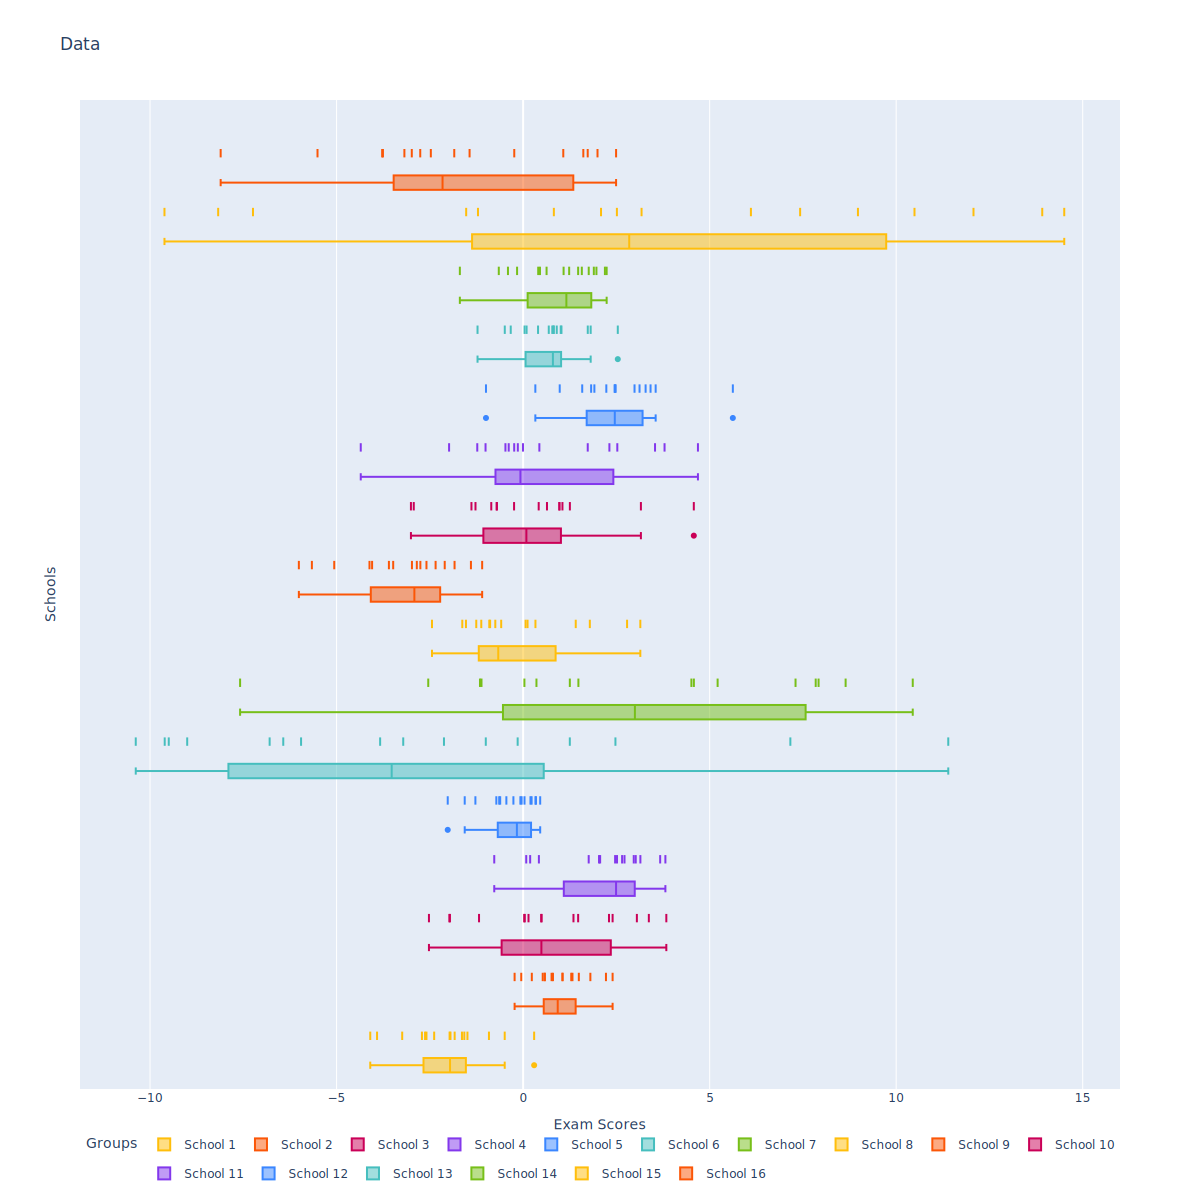
\includegraphics[width=\columnwidth]{files/data.pdf}}
    \caption{\textbf{Example of our exam-scores dataset.} Each school is a different group of student scores. The relative quality of a score cannot be inferred without knowing the distribution of scores in the school.}
    \label{exam-score}
    \end{center}
    \vskip -0.2in
\end{figure}

Suppose we wanted to model the exam scores of students from different schools. Our model must separate the school-level effect (the group factor) from the student-level effect (the instance factor). We define the following generative model:

$$x_{ik} = 2 ~ \mu_i +  (\sigma^2_i + 1) v_{ik}, ~ i \in 1:N, ~ k \in 1:K_i$$

where $x_{ij}$ is the student score, $u_i = (\mu_i, \sigma_i)$ is the school-level effect, $v_{ij}$ is the student-level effect. We assume a $\mathcal{N} (0, 1)$ prior distribution for the latent variables.

We first sample the model to generate a dataset ($N = 32,768, ~ K_i \sim \mathrm{Poisson} (16) + 8$) and then use the same model as the generative model in our Variational Autoencoder, instead of a neural network. The figure below shows what the data looks like.

Looking at the data, it is easy to see that this model is entangled, because the relative performance $v$ of a student within their own school, given their absolute score $x$, depends on the distribution of scores within the school $u$.

\section{Context-Aware Variational Autoencoder (CxVAE)}

We propose a new model which can perform well on datasets generated from entangled group and instance variable. We call our model the Context-Aware Variational Autoencoder. Our model comprises the following changes with respect to the standard GVAE:

\begin{enumerate}
    \item The group encoder is implemented as a Deep Sets network \citep{Zaheer2017DeepS}. The encoder has the following form:
    $$\mu, \Sigma = E_u (\mathbf{x}) = E^B_u \left( \sum_{k=1}^K E^A_u (x_k)\right)$$
    where $E^A_u, E^B_u$ are two neural networks.
    \item The variational instance posterior is dependent on the inferred group variable:
    $$q(u, \mathbf{v} | \mathbf{x}) = q(u | \mathbf{x}) \prod_{k=1}^K q(v_k | x_k, u)$$
    In practice, our instance encoder takes as input a vector concatenating $x_k$ and $u$. This idea is not new, and has been used previously in sequence disentanglement \citep{Li2018DisentangledSA}. This allows the instance encoder to differentiate the between observations with similar values but which come from different groups.
    \item We propose a regularization objective similar to the one in \citet{Nmeth2020AdversarialDW}, but whereby we minimize \textit{the mutual information between one inferred instance variable and all the other observations in the group}. More precisely, our objective is to minimize $I_r (\mathbf{x}_{-k}, v_k)$ where $r(v_k | \mathbf{x}_{-k}) = q(v_k | x_k, u)$. Following the same approximation as in \citet{Nmeth2020AdversarialDW}, the objective takes the following form:
    \begin{align}
        \begin{split}
            I_{r} (\mathbf{x}_{-k}, v_k) &\approx \max_{T} ~ \mathbb{E}_{r(\mathbf{x}_{-k}, v_k)} [T(\mathbf{x}_{-k}, v_k)] \\ - \log &\mathbb{E}_{r(\mathbf{x}_{-k}) r(v_k)} [\exp T(\mathbf{x}_{-k}, v_k)]
        \end{split}
    \end{align}
    $T$ is implemented as a Deep Sets neural network for the observations, with the instance code concatenated in the middle:
    $$T(\mathbf{x}_{-k}, v_k) = T^\beta \left(v_k, \frac{1}{K} \sum_{l=1, ~ l \neq k}^K T^\alpha (x_l) \right)$$
    Again, the expectations are computed by sampling:
    \begin{itemize}
        \item To sample $r(x, v)$, first choose a group $i$, then choose one instance from that group $k \in K_i$. $\mathbf{x}_{i,-k}$ will be all the observations in the group apart from $k$, and $v_k$ will be sampled from $q(v | x_{ik})$.
        \item To sample $r(\mathbf{x}_{-k})r(v_k)$, choose two groups $i, j$ and two instances in each group $k \in K_i, ~ l \in K_j$. Take $\mathbf{x}_{i, -k}$ for $\mathbf{x}_{-k}$ and sample $q(v | x_{jl})$. 
    \end{itemize}
    
    This regularization objective also minimizes the mutual information between the inferred instance variables and the true data generating group variable, but uses as a proxy for the latter all but one of the observations in the group, instead of just one observation.
\end{enumerate}

\section{Measuring Disentanglement}


\subsection{Probing $u$ and $\mathbf{v}$}

Our first evaluation metric is a direct application of the definition of disentanglement; that a given representation should capture as much information as possible about the corresponding data-generating factor,  and as little as possible about the other factors \citep{Locatello2020WeaklySupervisedDW}.  In the case of group-instance,  the inferred group variable $\hat{u}$, for example, should be maximally predictive of the data-generating group factor $u$, and minimally predictive of the set of instance factors $\mathbf{v}$

However, not all combinations of inferred latents and data-generating factors are worth analysing. As pointed out by \citet{Nmeth2020AdversarialDW}, the failure case we are trying to prevent in group-instance disentanglement is that the inferred instance variables $\hat{\mathbf{v}}$ might learn information pertaining to the data-generating group factor $u$. Other cases, such that the inferred group variable might learn to represent instance information, are not possible because of the structure of the variational model. The group encoder is an order-agnostic accumulation of input observations and the instance encoder is applied separately to each observation (so no way for information from observation $x_l$ to bleed into instance variable $\hat{v}_k$).

Thus, the metric is computed as follows: at training time, we learn two regressors, called probes,  to predict the data-generating group factor $u$: one probe takes as input the inferred group variable $\hat{u}$ and the other takes as input the set of inferred instance variables $\hat{\mathbf{v}}$. The prediction error rate of these regressors on the holdout set gives the disentanglement metric; the more disentangled the representation is, the lower the error of the $u$-probe and the higher the error of the $v$-probe. Since we are using a synthetic dataset for evaluation, we can measure the mean squared error directly between the prediction and the ground-truth group factor.

Training predictors on latent representations is a universal approach for evaluating disentanglement.  In particular, \citet{Bouchacourt2018MultiLevelVA, Nmeth2020AdversarialDW} have a very similar setup to ours, the only difference being that they use a classifier instead of a regressor. This is because they evaluate on real data whose ground-truth factors are unknown, so they use human lables as a proxy.

\subsection{Unsupervised Translation}

\begin{figure}[t]
    \vskip 0.2in
    \begin{center}
\begin{subfigure}{0.49\columnwidth}
    \includegraphics[width=\textwidth]{files/trans_ours.pdf}
    \caption{CxVAE}
\end{subfigure}
\hfill
\begin{subfigure}{0.49\columnwidth}
    \includegraphics[width=\textwidth]{files/trans_theirs.pdf}
    \caption{ML-VAE}
\end{subfigure}
    \caption{\textbf{Unsupervised translation with our CxVAE and the ML-VAE}.  The task is to generate a set of observations with the instance variables or the source group and the group variable of the target group. Visual inspection suggests that our model better captures the mean and variance of the target group.}
    \label{fig:trans}
    \end{center}
    \vskip -0.2in
\end{figure}

Unsupervised translation is the process of transforming an observation by changing its group code while keeping its instance code fixed. This is a primary downstream task for disentangled representations because it requires a clean separation between the group and instance representations \citep{Tenenbaum2000SeparatingSA}. Therefore, it can be used to quantify the quality of disentanglement.

Formally, let $i, j$ be the indices of the source and target group, respectively. Translation involves sampling a group of instance codes from the source group $q(\mathbf{v}_i | \mathbf{x}_i)$ and a group code from the target group $q(u_j | \mathbf{x}_j)$. Then, we generate the translated observations by combining each instance code with the group code $p(x'_{k} | \hat{u}_j, \hat{\mathbf{v}}_j)$. An example of translation comparing our CxVAE with the ML-VAE \citep{Bouchacourt2018MultiLevelVA} can be seen in \cref{fig:trans}.

We measure the translation quality by taking the mean squared error between the translation performed with each model and the ground-truth translation computed using the true data-generating process.

\section{Experiments}

\begin{figure}[t]
\vskip 0.2in
\begin{center}
\centerline{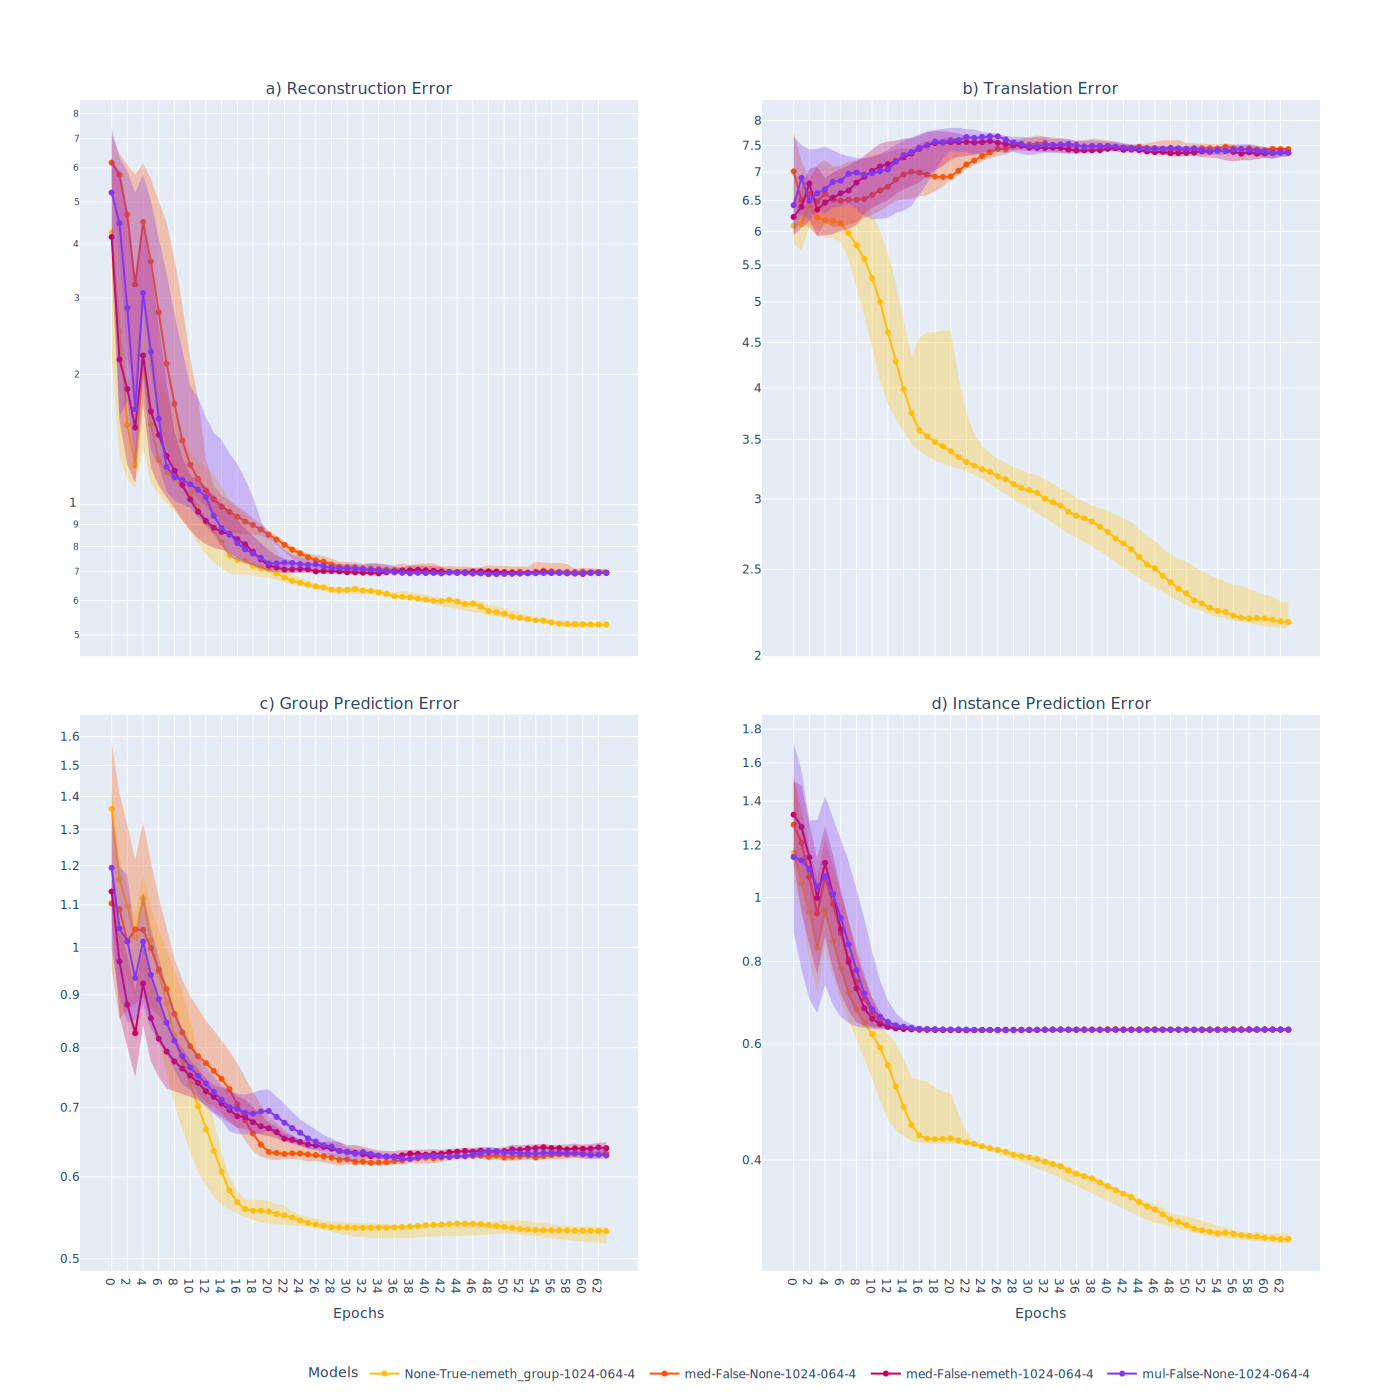
\includegraphics[width=\columnwidth]{files/results.pdf}}
\caption{Our CxVAE produces considerable improvements over the state-of-the-art in every disentanglement metric considered: holdout reconstruction error (\textbf{lower is better}), translation error (\textbf{lower is better}), $u$-probing (\textbf{lower is better}) and $\mathbf{v}$-probing (\textbf{higher is better}).  We show box-plots for the distribution of scores over 100 random initialisations. }
\label{fig:results}
\end{center}
\vskip -0.2in
\end{figure}

\begin{figure}[t]
\vskip 0.2in
\begin{center}
\centerline{\includegraphics[width=\columnwidth]{files/ablation.pdf}}
\caption{\textbf{Ablation study.} Replacing any novel component of our CxVAE with an existing alternative leads to worse performance. Note that the largest reduction in performance is brought by making the instance encoder unconditional. The next largest reduction is caused by changing the regularization, followed by using a less expressive group encoder.}
\label{fig:ablation}
\end{center}
\vskip -0.2in
\end{figure}

\begin{figure*}[t]
\vskip 0.2in
\begin{center}
\centerline{\includegraphics[width=\textwidth]{files/xy_ratio.pdf}}
\caption{\textbf{The performance gain of our CxVAE increases with more confounding.} We show disentanglement on datasets generated with different values of the $\gamma$ hyper-parameter, controlling the ratio of magnitudes between the confounded and unconfounded components of the instance factor. For low values of $\gamma$ the instance factor is not confounded and so the CxVAE and GVAE perform equally well. However, as $\gamma$ increases, GVAE performs more poorly.}
\label{fig:xy}
\end{center}
\vskip -0.2in
\end{figure*}

\begin{figure*}[t]
\vskip 0.2in
\begin{center}
\centerline{\includegraphics[width=\textwidth]{files/uv_ratio.pdf}}
\caption{\textbf{Similar magnitudes of the group and instance factors produces a dip in the performance of the GVAE. } We show disentanglement on exam-score datasets generated with different values of the $\lambda$ hyper-parameter, controlling the ratio of magnitudes between the group and instance factors.  The greatest gap in performance between our CxVAE and the GVAE occurs when $\lambda=0.5$ when the magnitude of the variation across groups is equal to the magnitude within groups.  Too small (weak groups) or too large (strong groups) values of $\lambda$ lead to a normal autoencoding problem.}
\label{fig:uv}
\end{center}
\vskip -0.2in
\end{figure*}

In the first experiment, we compare our CxVAE with the state-of-the-art in group-instance disentanglement, namely the Multi-Level VAE (ML-VAE) \citep{Bouchacourt2018MultiLevelVA}, the Group VAE (GVAE) \citep{Hosoya2019GroupbasedLO} and the Adversarial GVAE (GVAE-AD) \citep{Nmeth2020AdversarialDW}.

We generate a dataset with $N = 65,536$ groups. The size of each group is distributed according to a Poisson distribution $K_i \sim 8 + \mathrm{Poisson}(16)$. We train each model for 64 epochs, and use the last 10 epochs for evaluation. Additionally, we run the experiment for 10 different random seeds initialisations, both for the data generating process and the networks. We use the same 10 seeds to compare. This gives us 100 measurements to plot in \cref{fig:results}.

\paragraph{Results} Our CxVAE produces considerable improvements over the state-of-the-art in every disentanglement metric considered (\cref{fig:results}). While the scores of the existing methods cluster together, the gap between them and the CxVAE is larger than any 95\% confidence interval. It is also interesting to note how CxVAE produces a smaller reconstruction error on the holdout dataset, suggesting that disentangled representations generalise better to unseen groups.

\subsection{Ablation Study}

In order to quantify the contribution of each of the modifications that comprise our proposed model, we perform an ablation study whereby we measure the decrease in performance resulting from replacing a proposed component with an existing alternative. For example, when considering the group encoder, we include in the comparison two hybrid models based on the CxVAE: one of them has a product of normals encoder as in the ML-VAE, while the other has an averaging encoder as in the GVAE.  For the instance encoder, the alternative is to have no conditioning on the group variable. For the regularization, we compare with the adversarial loss of GVAE+AD and with no regularization at all. The results of the experiment are displayed in \cref{fig:ablation}.

\paragraph{Results} The full CxVAE has a better performance than any alternative configuration.  In particular, the choice of a conditional instance encoder brings the largest improvement in performance, followed by the regularization objective, then the group encoder.

\subsection{Degree of Confounding}

Is the increased performance of our CxVAE solely due to the confounded data-generating process, or is it simply a better all-round model? To answer this, we create different exam-scores datasets with different degrees of confounding.  We do this by making the data 2-dimensional, with one dimension being confounded and the other being controlled only by the instance variable, and then trading off the magnitude of one to the other. Our new data generating process is the following:

\begin{equation}
x_{ik} = \begin{bmatrix}
u_i + \gamma a_{ik}\\
(1 - \gamma) b_{ik}
\end{bmatrix}, ~ v_{ik} = \begin{bmatrix}
a_{ik} \\ b_{ik}
\end{bmatrix}
\end{equation}

where $a_{ik}$ is the dimension of the instance factor confounded by the group factor, while $b_{ik}$ is the unconfounded dimension. The trade-off is controlled using a hyper-parameter $\gamma \in [0,1]$. For low values of $\gamma$, the confounded variable should explain a small amount of the variation within groups. In that case, our CxVAE should not perform much better than existing methods, if our hypothesis about the relationship between CxVAE and confounding is correct.  Large values of $\gamma$ correspond to the settings we have already tested, so the performance gap should be large.

\paragraph{Results} The measurements displayed in \cref{fig:xy} confirm our expectations. For low values of $\gamma$ the performance of our CxVAE is evenly matched to the GVAE.  As $\gamma$ increases, CxVAE scores remain relatively stable while GVAE scores decrease substantially.  It is clear that the degree of confounding in the dataset explains the performance gain that we see in the CxVAE. 

\subsection{Stronger Group or Stronger Instance}

It is interesting to observe how changing the relative strength of the group and instance ground-truth factors in the dataset impacts differentely the disentanglement in our CxVAE and GVAE. Since our data is generated by a simple mixed model, we can adjust the data-generating process as follows:

\begin{equation}
x_{ik} = \lambda u_i + (1 - \lambda) v_{ik}
\end{equation}

where $\lambda \in [0, 1]$ is a hyper-parameter controlling the strength of the group factor $\mu_i$ relative to the instance factor $v_{ik}$. 

We expect that different values for $\lambda$ would change the characteristics of the disentanglement problem. A low value $\lambda \approx 0$ would generate a dataset with weak grouping that is virtually i.i.d. and that a normal autoencoder could represent. A large value $\lambda \approx 1$ would generate a dataset with strong groups where the observations within a group are noisy copies of one another, a setting that can also be solved by simple autoencoding.  A middle value $\lambda \approx 0.5$ would evenly match the impact of the group and instance variables. Here we expect the performance gain of the CxVAE over competing methods to be greatest.

\paragraph{Results} Looking at \cref{fig:uv} we note, as expected, that the largest performance gain of the CxVAE occurs at $\lambda = 0$. Specifically, while the performance of the CxVAE increases steadily as $\lambda$ goes from 0 to 1,  the scores of GVAE dip significantly around $\lambda = 0.5$. Translation and $\mathbf{v}$-probing are most sensitive to the decrease in performance of the GVAE. We also observe that the scores generally increase with $\lambda$ even as the average magnitude of the data remains constant, possibly because for $\lambda \approx 0$ the group encoder cannot be used for learning, and thus expressiveness is lost.

\section{Related Work}

\section{Conclusions}

\bibliography{main}
\bibliographystyle{icml2022}


%%%%%%%%%%%%%%%%%%%%%%%%%%%%%%%%%%%%%%%%%%%%%%%%%%%%%%%%%%%%%%%%%%%%%%%%%%%%%%%
%%%%%%%%%%%%%%%%%%%%%%%%%%%%%%%%%%%%%%%%%%%%%%%%%%%%%%%%%%%%%%%%%%%%%%%%%%%%%%%
% APPENDIX
%%%%%%%%%%%%%%%%%%%%%%%%%%%%%%%%%%%%%%%%%%%%%%%%%%%%%%%%%%%%%%%%%%%%%%%%%%%%%%%
%%%%%%%%%%%%%%%%%%%%%%%%%%%%%%%%%%%%%%%%%%%%%%%%%%%%%%%%%%%%%%%%%%%%%%%%%%%%%%%
\newpage
\appendix
\onecolumn
\section{You \emph{can} have an appendix here.}

You can have as much text here as you want. The main body must be at most $8$ pages long.
For the final version, one more page can be added.
If you want, you can use an appendix like this one, even using the one-column format.
%%%%%%%%%%%%%%%%%%%%%%%%%%%%%%%%%%%%%%%%%%%%%%%%%%%%%%%%%%%%%%%%%%%%%%%%%%%%%%%
%%%%%%%%%%%%%%%%%%%%%%%%%%%%%%%%%%%%%%%%%%%%%%%%%%%%%%%%%%%%%%%%%%%%%%%%%%%%%%%


\end{document}


% This document was modified from the file originally made available by
% Pat Langley and Andrea Danyluk for ICML-2K. This version was created
% by Iain Murray in 2018, and modified by Alexandre Bouchard in
% 2019 and 2021 and by Csaba Szepesvari, Gang Niu and Sivan Sabato in 2022. 
% Previous contributors include Dan Roy, Lise Getoor and Tobias
% Scheffer, which was slightly modified from the 2010 version by
% Thorsten Joachims & Johannes Fuernkranz, slightly modified from the
% 2009 version by Kiri Wagstaff and Sam Roweis's 2008 version, which is
% slightly modified from Prasad Tadepalli's 2007 version which is a
% lightly changed version of the previous year's version by Andrew
% Moore, which was in turn edited from those of Kristian Kersting and
% Codrina Lauth. Alex Smola contributed to the algorithmic style files.
